\documentclass[10pt,landscape]{article}
\usepackage{multicol}
\usepackage{calc}
\usepackage{ifthen}
\usepackage[landscape]{geometry}
\usepackage{listings}
\usepackage{amsmath,amsthm,amsfonts,amssymb}
\usepackage{mathtools}
\usepackage{color,graphicx,overpic}
\usepackage{hyperref}
\usepackage[dvipsnames]{xcolor}

\usepackage{MnSymbol}
\usepackage{graphicx}
\usepackage{wrapfig}
\usepackage{tikz}

\usepackage{blindtext}

% This sets page margins to .1 inch if using letter paper, and to 1cm
% if using A4 paper. (This probably isn't strictly necessary.)
% If using another size paper, use default 1cm margins.
\ifthenelse{\lengthtest { \paperwidth = 11in}}
    { \geometry{top=0.2in,left=0.2in,right=0.2in,bottom=0.2in} }
    {\ifthenelse{ \lengthtest{ \paperwidth = 297mm}}
        {\geometry{top=1cm,left=1cm,right=1cm,bottom=1cm} }
        {\geometry{top=1cm,left=1cm,right=1cm,bottom=1cm} }
    }

% Turn off header and footer
\pagestyle{empty}

% Redefine section commands to use less space
\makeatletter
\renewcommand{\section}{\@startsection{section}{1}{0mm}%
                                {-1ex plus -.5ex minus -.2ex}%
                                {0.5ex plus .2ex}%x
                                {\normalfont\large\bfseries}}
\renewcommand{\subsection}{\@startsection{subsection}{2}{0mm}%
                                {-1ex plus -.5ex minus -.2ex}%
                                {0.5ex plus .2ex}%
                                {\normalfont\normalsize\bfseries}}
\renewcommand{\subsubsection}{\@startsection{subsubsection}{3}{0mm}%
                                {-1ex plus -.5ex minus -.2ex}%
                                {0.5ex plus .2ex}%
                                {\normalfont\footnotesize\bfseries}}
\makeatother

% Itemize to use less space
\usepackage{enumitem}
\setlist{leftmargin=*, nosep}
\setenumerate{nosep}

% Define BibTeX command
\def\BibTeX{{\rm B\kern-.05em{\sc i\kern-.025em b}\kern-.08em
    T\kern-.1667em\lower.7ex\hbox{E}\kern-.125emX}}

% Don't print section numbers
\setcounter{secnumdepth}{0}


\setlength{\parindent}{0pt}
\setlength{\parskip}{0pt plus 0.5ex}

%My Environments
\newtheorem{example}[section]{Example}

\newcommand{\Blue}[1]{\noindent{\textcolor{Blue}{\textbf{#1}}}:}
\newcommand{\Red}[1]{\noindent{\textcolor{BrickRed}{\textbf{#1}}}:}
\newcommand{\Green}[1]{\noindent{\textcolor{PineGreen}{\textbf{#1}}}:}
\newcommand{\Hint}[1]{\noindent{\textcolor{Orange}{#1}}}

\newcommand*{\eg}{e.g.\@\xspace}
\newcommand*{\ie}{i.e.\@\xspace}
\newcommand*{\Eg}{E.g.\@\xspace}
\newcommand*{\Ie}{I.e.\@\xspace}
\newcommand*{\esp}{esp.\@\xspace}
\newcommand*{\wrt}{\ifmmode \stext{w.r.t.} \else w.r.t.\@\xspace \fi}


\usepackage{draftwatermark}
% Configure the watermark
\SetWatermarkText{Made with love by \texttt{junruren}} % Set the watermark text
\SetWatermarkScale{2}            % Adjust the scale of the watermark
\SetWatermarkLightness{0.97}      % Set the lightness (closer to 1 is more faded)
% -----------------------------------------------------------------------

\begin{document}
\raggedright
\scriptsize

\begin{multicols}{4}
% multicol parameters
% These lengths are set only within the two main columns
%\setlength{\columnseprule}{0.25pt}
\setlength{\premulticols}{1pt}
\setlength{\postmulticols}{1pt}
\setlength{\multicolsep}{1pt}
\setlength{\columnsep}{2pt}

\subsubsection{Supply and Demand}

\Red{Demand} how much consumers will buy at a particular price; describes consumers' willingness to pay (WTP).
\fbox{$Q_d = a - b \cdot P$}

\Red{Supply} how much producers will provide at a particular price; describes producers' willingness to accept (WTA) /
the industry's aggregate marginal cost curve (\ie Market supply is the \underline{sum} of the
individual firm supply curves).
\fbox{$Q_s = c + d \cdot P$}

\Hint{\underline{Remember} to always check whether we need to \underline{invert} a given function!}
\Blue{Competitive Markets} Individual firms and consumers don't affect prices (\ie they have no market power and are
price takers)

\Red{Competitive Market Equilibrium} \fbox{$Q^* = Q_s (P^*) = Q_d (P^*)$}
In these markets, \Hint{prices are determined} by:
\begin{itemize}
    \item the \Blue{``marginal buyer'' $P^* = WTP$} who would leave the market if the price were any higher, and
    \item the \Blue{``marginal seller'' $P^* = WTA$} who would leave the market if the price were any lower
\end{itemize}

\Blue{Producer Surplus (PS)} = Revenue - Total WTA = Revenue - Total Variable Cost (area below price and above supply.)

Without market power, \Hint{firm-level inverse demand curve is perfectly elastic} (\ie horizontal) \Hint{at the market
price.} Market sets \fbox{$MR(Q) = P$}. \Hint{Firm's supply curve is its MC curve}. Firm profit \textbf{maximized} when:
\fbox{$\text{Market } P = MR(Q^*) = MC(Q^*)$}, provided the firm is operating at all.
\textit{Not to be confused with
the MR discussed in H1 Monopoly Pricing!}

\Red{First Welfare Theorem} Competitive markets are \textbf{efficient} (\ie they maximize total surplus = CS + PS).
\begin{itemize}
    \item Assumes no distortions such as market power, info frictions, or \textit{externalities}.
    \item Under perfect competition, all trades involving consumers who value the good more than the marginal cost associated with producing an additional unit of the good are realized.
\end{itemize}

\Blue{Welfare is maximized} by the perfectly competitive outcome when there are not externalities.
To maximize total welfare, we want
\begin{itemize}
    \item Consumers get: $CS = \frac{1}{2} (a - P^*)Q^*$
    \item Producers get: $PS = \frac{1}{2} (P^* - c)Q^*$
\end{itemize}

\begin{multicols}{2}
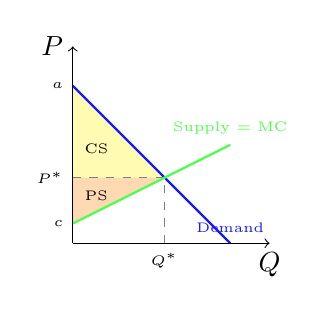
\begin{tikzpicture}
    % CS
    \fill[yellow!30] (0, 0.83) -- (1.16, 0.83) -- (0, 2) -- cycle;

    %PS
    \fill[orange!30] (0, 0.25) -- (0, 0.83) -- (1.16, 0.83) -- cycle;

    \draw[dashed,gray] (0, 0.83) -- (1.16, 0.83);
    \draw[dashed,gray] (1.16, 0) -- (1.16, 0.83);
    \draw[thick,blue!90] (0,2) -- (2,0) node[anchor=south] {\tiny Demand}; % Demand curve
    \draw[thick, green!70] (0,0.25) -- (2,1.25) node[anchor=south] {\tiny Supply = MC}; % Supply curve
    % Draw axes
    \draw[->] (0,0) -- (2.5,0) node[anchor=north] {$Q$};
    \draw[->] (0,0) -- (0,2.5) node[anchor=east] {$P$};
    
    % Label values
    \node[anchor=north] at (1.16,0) {\tiny $Q^*$};
    \node[anchor=east] at (0,0.83) {\tiny $P^*$};
    \node[anchor=east] at (0,0.25) {\tiny $c$};
    \node[anchor=east] at (0,2) {\tiny $a$};
    \node at (0.3,1.2) {\tiny CS};
    \node at (0.3,0.6) {\tiny PS};

\end{tikzpicture}
Competitive markets maximize total surplus.
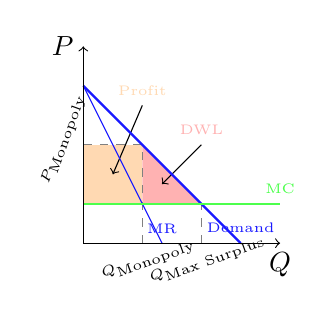
\begin{tikzpicture}
    %DWL
    \fill[red!30] (0.75, 0.5) -- (0.75, 1.25) -- (1.5, 0.5) -- cycle;
    \draw[<-] (1, 0.75) -- (1.5, 1.25) node[anchor=south,red!30] {\tiny DWL};

    %Profit
    \fill[orange!30] (0, 0.5) -- (0, 1.25) -- (0.75, 1.25) -- (0.75, 0.5) -- cycle;
    \draw[<-] (0.375, 0.875) -- (0.75, 1.75) node[anchor=south,orange!30] {\tiny Profit};

    \draw[dashed,gray] (0, 1.25)  -- (0.75, 1.25); % P_monopoly dashed line
    \draw[dashed,gray] (0.75, 0) -- (0.75, 1.25); % Q_monopoly dashed line
    \draw[dashed,gray] (1.5, 0) -- (1.5, 0.5); % Q_max surplus dashed line
    \draw[thick,blue!90] (0,2) -- (2,0) node[anchor=south] {\tiny Demand}; % Demand curve
    \draw[blue!90] (0,2) -- (1,0) node[anchor=south] {\tiny MR}; % MR curve
    \draw[thick, green!70] (0,0.5) -- (2.5,0.5) node[anchor=south] {\tiny MC}; % Supply curve
    % Draw axes
    \draw[->] (0,0) -- (2.5,0) node[anchor=north] {$Q$};
    \draw[->] (0,0) -- (0,2.5) node[anchor=east] {$P$};
    
    % Label values
    \node[anchor=north, rotate=20] at (0.75,0) {\tiny $Q_{\text{Monopoly}}$};
    \node[anchor=north, rotate=20] at (1.5,0) {\tiny $Q_{\text{Max Surplus}}$};
    \node[anchor=east, rotate=70] at (0,2) {\tiny $P_{\text{Monopoly}}$};

\end{tikzpicture}
Distortion \eg: Pricing with market power
\end{multicols}

\Red{Deadweight Loss (DWL)} Lost surplus due to a distortion away from perfect competition. \fbox{DWL = CS + PS - TS} \ie Maximum surplus - Achieved surplus. DWL offers an opportunity to ``grow the pie'', represents the value proposition for many firms.

\Green{In the left graph} DWL will be generated
\begin{itemize}
    \item if $Q < Q^*$ because there will be consumers that value the product at above the marginal cost
    \item if $Q > Q^*$ because there will be consumers consuming the product even though their $WTP < MC$
\end{itemize}

\Red{Cost Shock} if one side of the market is highly elastic, then they can avoid shocks (and pass on any taxes / transation fees).
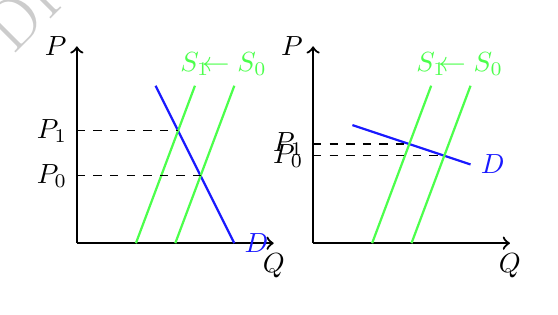
\begin{tikzpicture}

    % LEFT GRAPH
    % Axes
    \draw[thick,->] (0,0) -- (2.5,0) node[anchor=north] {$Q$};
    \draw[thick,->] (0,0) -- (0,2.5) node[anchor=east] {$P$};
    
    % Demand Curve
    \draw[thick,blue!90] (1,2) -- (2,0) node[right] {$D$};
    
    % Supply Curves
    \draw[thick,green!70] (1.25,0) -- (2,2) node[above] {$\leftarrow S_0$};
    \draw[thick,green!70] (0.75,0) -- (1.5,2) node[above] {$S_1$};
    
    % Price levels
    \draw[dashed] (0,1.4285714286) -- (1.2857142857,1.4285714286) node[left] at (0,1.4285714286) {$P_1$};
    \draw[dashed] (0,0.8571428571) -- (1.5714285714,0.8571428571) node[left] at (0,0.8571428571) {$P_0$};
    
    % RIGHT GRAPH
    \begin{scope}[shift={(3,0)}] % Shift to the right for the second plot
    % Axes
    \draw[thick,->] (0,0) -- (2.5,0) node[anchor=north] {$Q$};
    \draw[thick,->] (0,0) -- (0,2.5) node[anchor=east] {$P$};
    
    % Demand Curve
    \draw[thick,blue!90] (0.5,1.5) -- (2,1) node[right] {$D$};
    
    % Supply Curves
    \draw[thick,green!70] (1.25,0) -- (2,2) node[above] {$\leftarrow S_0$};
    \draw[thick,green!70] (0.75,0) -- (1.5,2) node[above] {$S_1$};
    
    % Price levels
    \draw[dashed] (0,1.2592592593) -- (1.2222222222,1.2592592593) node[left] at (0,1.2592592593) {$P_1$};
    \draw[dashed] (0,1.1111111111) -- (1.6666666667,1.1111111111) node[left] at (0,1.1111111111) {$P_0$};
    
    \end{scope}
\end{tikzpicture}

\end{multicols}
\end{document}